\documentclass[border=5pt]{standalone}
\usepackage{amsmath}
\usepackage{tikz}
\usetikzlibrary{positioning, fit, shapes, arrows}
\usetikzlibrary{chains}
\usetikzlibrary{calc}
\usetikzlibrary{decorations.pathmorphing}
\usetikzlibrary{decorations.pathreplacing}
\usetikzlibrary{shapes.multipart}
\usetikzlibrary{patterns}
\begin{document}

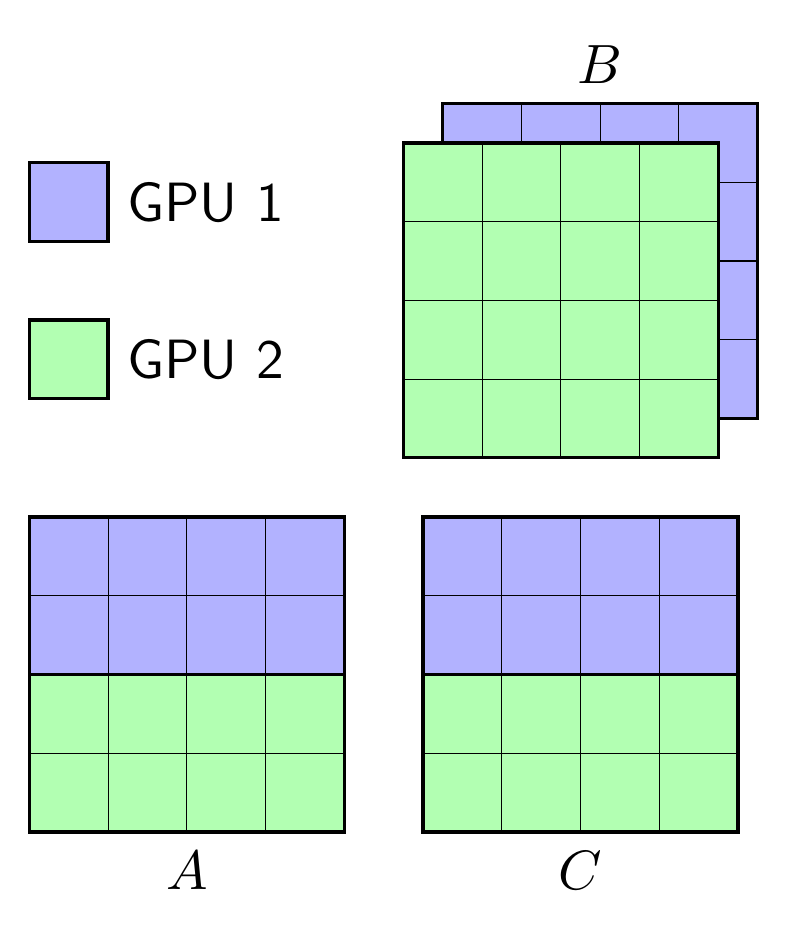
\begin{tikzpicture}[node distance=0.15 cm, font=\sffamily]

% A
\begin{scope}[xshift=-5cm]
  \fill[color=green!30, very thick] (0,0) rectangle (4,2);
  \fill[color=blue!30] (0,2) rectangle (4,4);
	\draw[very thick] (0,0) rectangle (4,2);
	\draw[very thick] (0,2) rectangle (4,4);

  \draw[step=1cm,black,thin] (0,0) grid (4,4);

  \node[anchor=north, scale=2] at (2,0) {$A$};
\end{scope}

% B1
\begin{scope}[yshift=5.25cm, xshift=.25cm]
  \fill[color=blue!30] (0,0) rectangle (4,4);
	\draw[very thick] (0,0) rectangle (4,4);

  \draw[step=1cm,black,thin] (0,0)grid(4,4);

  \node[anchor=south, scale=2] at (2,4) {$B$};
\end{scope}

% B1
\begin{scope}[yshift=4.75cm, xshift=-.25cm]
  \fill[color=green!30] (0,0) rectangle (4,4);
	\draw[very thick] (0,0) rectangle (4,4);

  \draw[step=1cm,black,thin] (0,0)grid(4,4);
\end{scope}

% C
\begin{scope}[]
  \fill[color=green!30, very thick] (0,0) rectangle (4,2);
  \fill[color=blue!30, very thick] (0,2) rectangle (4,4);
	\draw[very thick] (0,0) rectangle (4,2);
	\draw[very thick] (0,2) rectangle (4,4);

  \draw[step=1cm,black,thin] (0,0)grid(4,4);

  \node[anchor=north, scale=2] at (2,0) {$C$};
\end{scope}

% legende
\begin{scope}[yshift=5.5cm, xshift=-5cm]
  \begin{scope}[yshift=2cm]
    \fill[color=blue!30] (0,0) rectangle (1,1);
	  \draw[very thick] (0,0) rectangle (1,1);
    \node[anchor=west, scale=2] at (1,0.5) {GPU 1};
  \end{scope}
  \begin{scope}
    \fill[color=green!30] (0,0) rectangle (1,1);
	  \draw[very thick] (0,0) rectangle (1,1);
    \node[anchor=west, scale=2] at (1,0.5) {GPU 2};
  \end{scope}
\end{scope}

\end{tikzpicture}
\end{document}

